\documentclass[12pt]{report}
\usepackage{graphicx}
\usepackage[T1]{fontenc}
\usepackage[english]{babel}
\usepackage{amsmath,amssymb}
\usepackage[a4paper, total={6in, 8.3in}]{geometry}
\usepackage{siunitx}
\usepackage{hyperref}
\usepackage{array}
\usepackage{float}
\usepackage{overpic}

\begin{document}
\begin{titlepage}
    \centering
    \vspace*{2cm}
    \huge \textbf{Modal Analysis of a Rail Wheel}\\ 
    \vspace*{1cm}
    \Large \textbf{Advanced Dynamics of Mechanical Systems}\\
    \vspace{2.5cm}
    \Large
    \begin{flushright}
    Authors:\\
    \vspace{0.1cm}
    Andrea GALENDA\\Matteo FILIPPI\\Daniele FIRMANI\\Alessandro GORLA
    \end{flushright}
    \vspace{1cm}
    \vfill
    {\Large Academic Year 2023/2024\par}
\end{titlepage}

\newpage
\begin{abstract}
This report details the modal parameters identification of a rail wheel starting from real experimental data. The vibration measurements, obtained through a dynamo-metric impact hammer and twelve accelerometers, are used to generate Frequency Response Functions (FRFs). A best fitting procedure is then applied to extract the natural frequencies, modal damping, and reconstruct the mode shapes of the wheel.
\end{abstract}

\tableofcontents
\newpage

\chapter*{Theoretical Background: Cantilever Beam}
\addcontentsline{toc}{chapter}{Theoretical Background}
The fundamental objective of modal analysis is to derive the natural frequencies and mode shapes of a structure. Using a cantilever beam as a baseline analytical model, the standing wave solution is derived by applying appropriate boundary conditions (null displacement and rotation at the clamped end; moment and vertical force equilibrium at the free end). This yields an eigenvalue problem from which the structure's exact natural frequencies and continuous shape functions are computed.

Experimentally, Frequency Response Functions (FRFs) are measured for different input-output position pairs. By employing a multi-mode curve fitting method, these FRFs are approximated numerically to minimize the least-square error with the real experimental data. The modal parameters, such as natural frequencies and modal damping ratios, are extracted directly from the fitted FRFs. Finally, the mode shapes are reconstructed by evaluating the imaginary part of the FRFs at the resonant frequencies. This core theoretical foundation is directly applicable to the modal identification of much more complex physical systems.


\chapter{Rail Wheel Modal Analysis}
\section{Introduction}
This project consists of a modal parameters identification starting from real experimental data coming from vibration measurements of a rail wheel.
\begin{figure}[H]
    \centering
    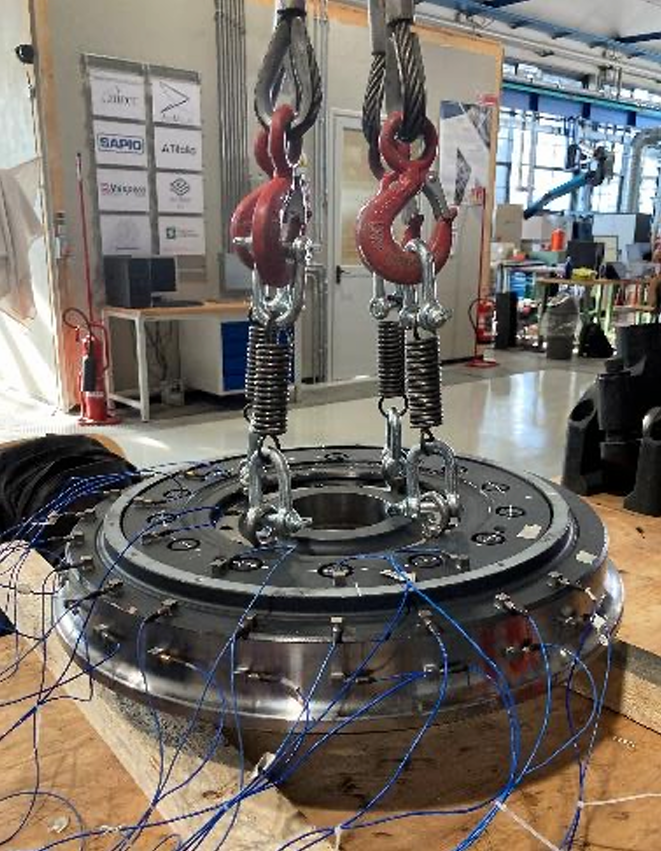
\includegraphics[width=0.5\linewidth]{Images/wheel.png}
    \caption{Experimental setup}
\end{figure}
\noindent
The wheel has been suspended through elastic supports and a dynamo-metric impact hammer has been leveraged to apply an axial load.\\
The output was measured by placing twelve accelerometers on half of the wheel exploiting the symmetry of the structure.\\
The resulting measurements have been used to generate a dataset containing twelve FRFs and their corresponding coherence functions.
\begin{figure}[H]
    \centering
    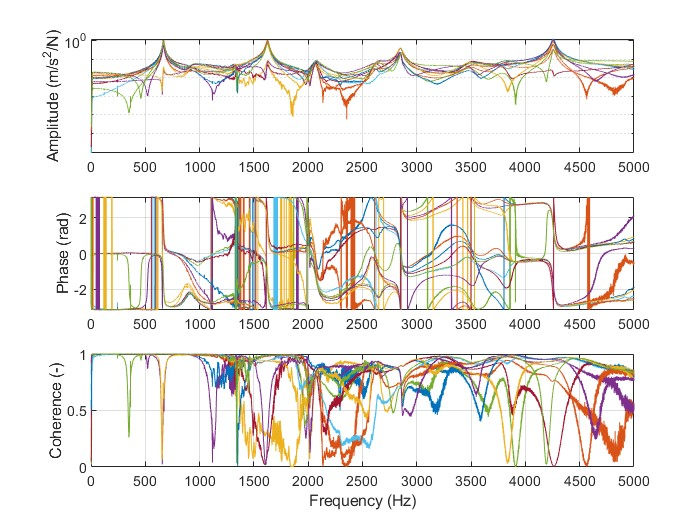
\includegraphics[scale=0.5]{Images/DataParteB.jpg}
    \caption{Experimental FRFs and coherence functions}
\end{figure}

\section{Modal parameters identification}
Numerical FRFs have to be computed starting from experimental data, exploiting an error minimisation procedure.

\subsection{Initial guesses estimation}
Starting from the data shown above, initial guesses are computed for the calculation of natural frequencies.\\
Indeed, the first two natural frequencies of each FRF have been computed, then the ones related to a non reasonable value of the coherence function have been deleted.\\
Finally, a mean of the remaining frequencies has been conducted for each mode. \\
The resulting eigenfrequencies are the following ones:\\
\begin{center}
    \begin{tabular}{c|c}
        \multicolumn{1}{c}{\textbf{Mode}} & \multicolumn{1}{c}{\textbf{Natural frequency [Hz]}}\\
        1 & 667.3 \\
        2 & 1625 \\
    \end{tabular}
\end{center}

\subsection{Best fitting procedure}
Once the initial guesses have been estimated, the minimization procedure can be applied. \\This procedure consists in a comparison between experimental and numerical FRFs; the latter ones computed according to the best fitting method.\\
Whenever the experimental FRFs do not show a clear peak at the eigenfrequencies, the coherence function suddenly drops.\\
Low values of the coherence function imply that the input and output signals are not actually correlated in that frequency range.\\
This happens close to an eigenfrequency and indicates that the system response is not affected by that specific mode, suggesting that the point could be a node of the mode associated with the eigenfrequency.\\
The resulting modal damping values are here reported:
\begin{center}
    \begin{tabular}{c|c}
        \multicolumn{1}{c}{\textbf{Mode}} & \multicolumn{1}{c}{\textbf{Modal damping values}}\\
        1 & 0.008 \\
        2 & 0.006 \\
    \end{tabular}
\end{center}

\subsection{Mode shapes reconstruction}
Once we have obtained the numerical FRFs, we can reconstruct the mode shapes using the following formula:
\begin{equation*}
\phi_i = Imag\left( G_{jk} \left(\omega _i \right) \right)
\end{equation*}
The reconstructed mode shapes are here reported:\\
\begin{figure} [H]
    \centering
    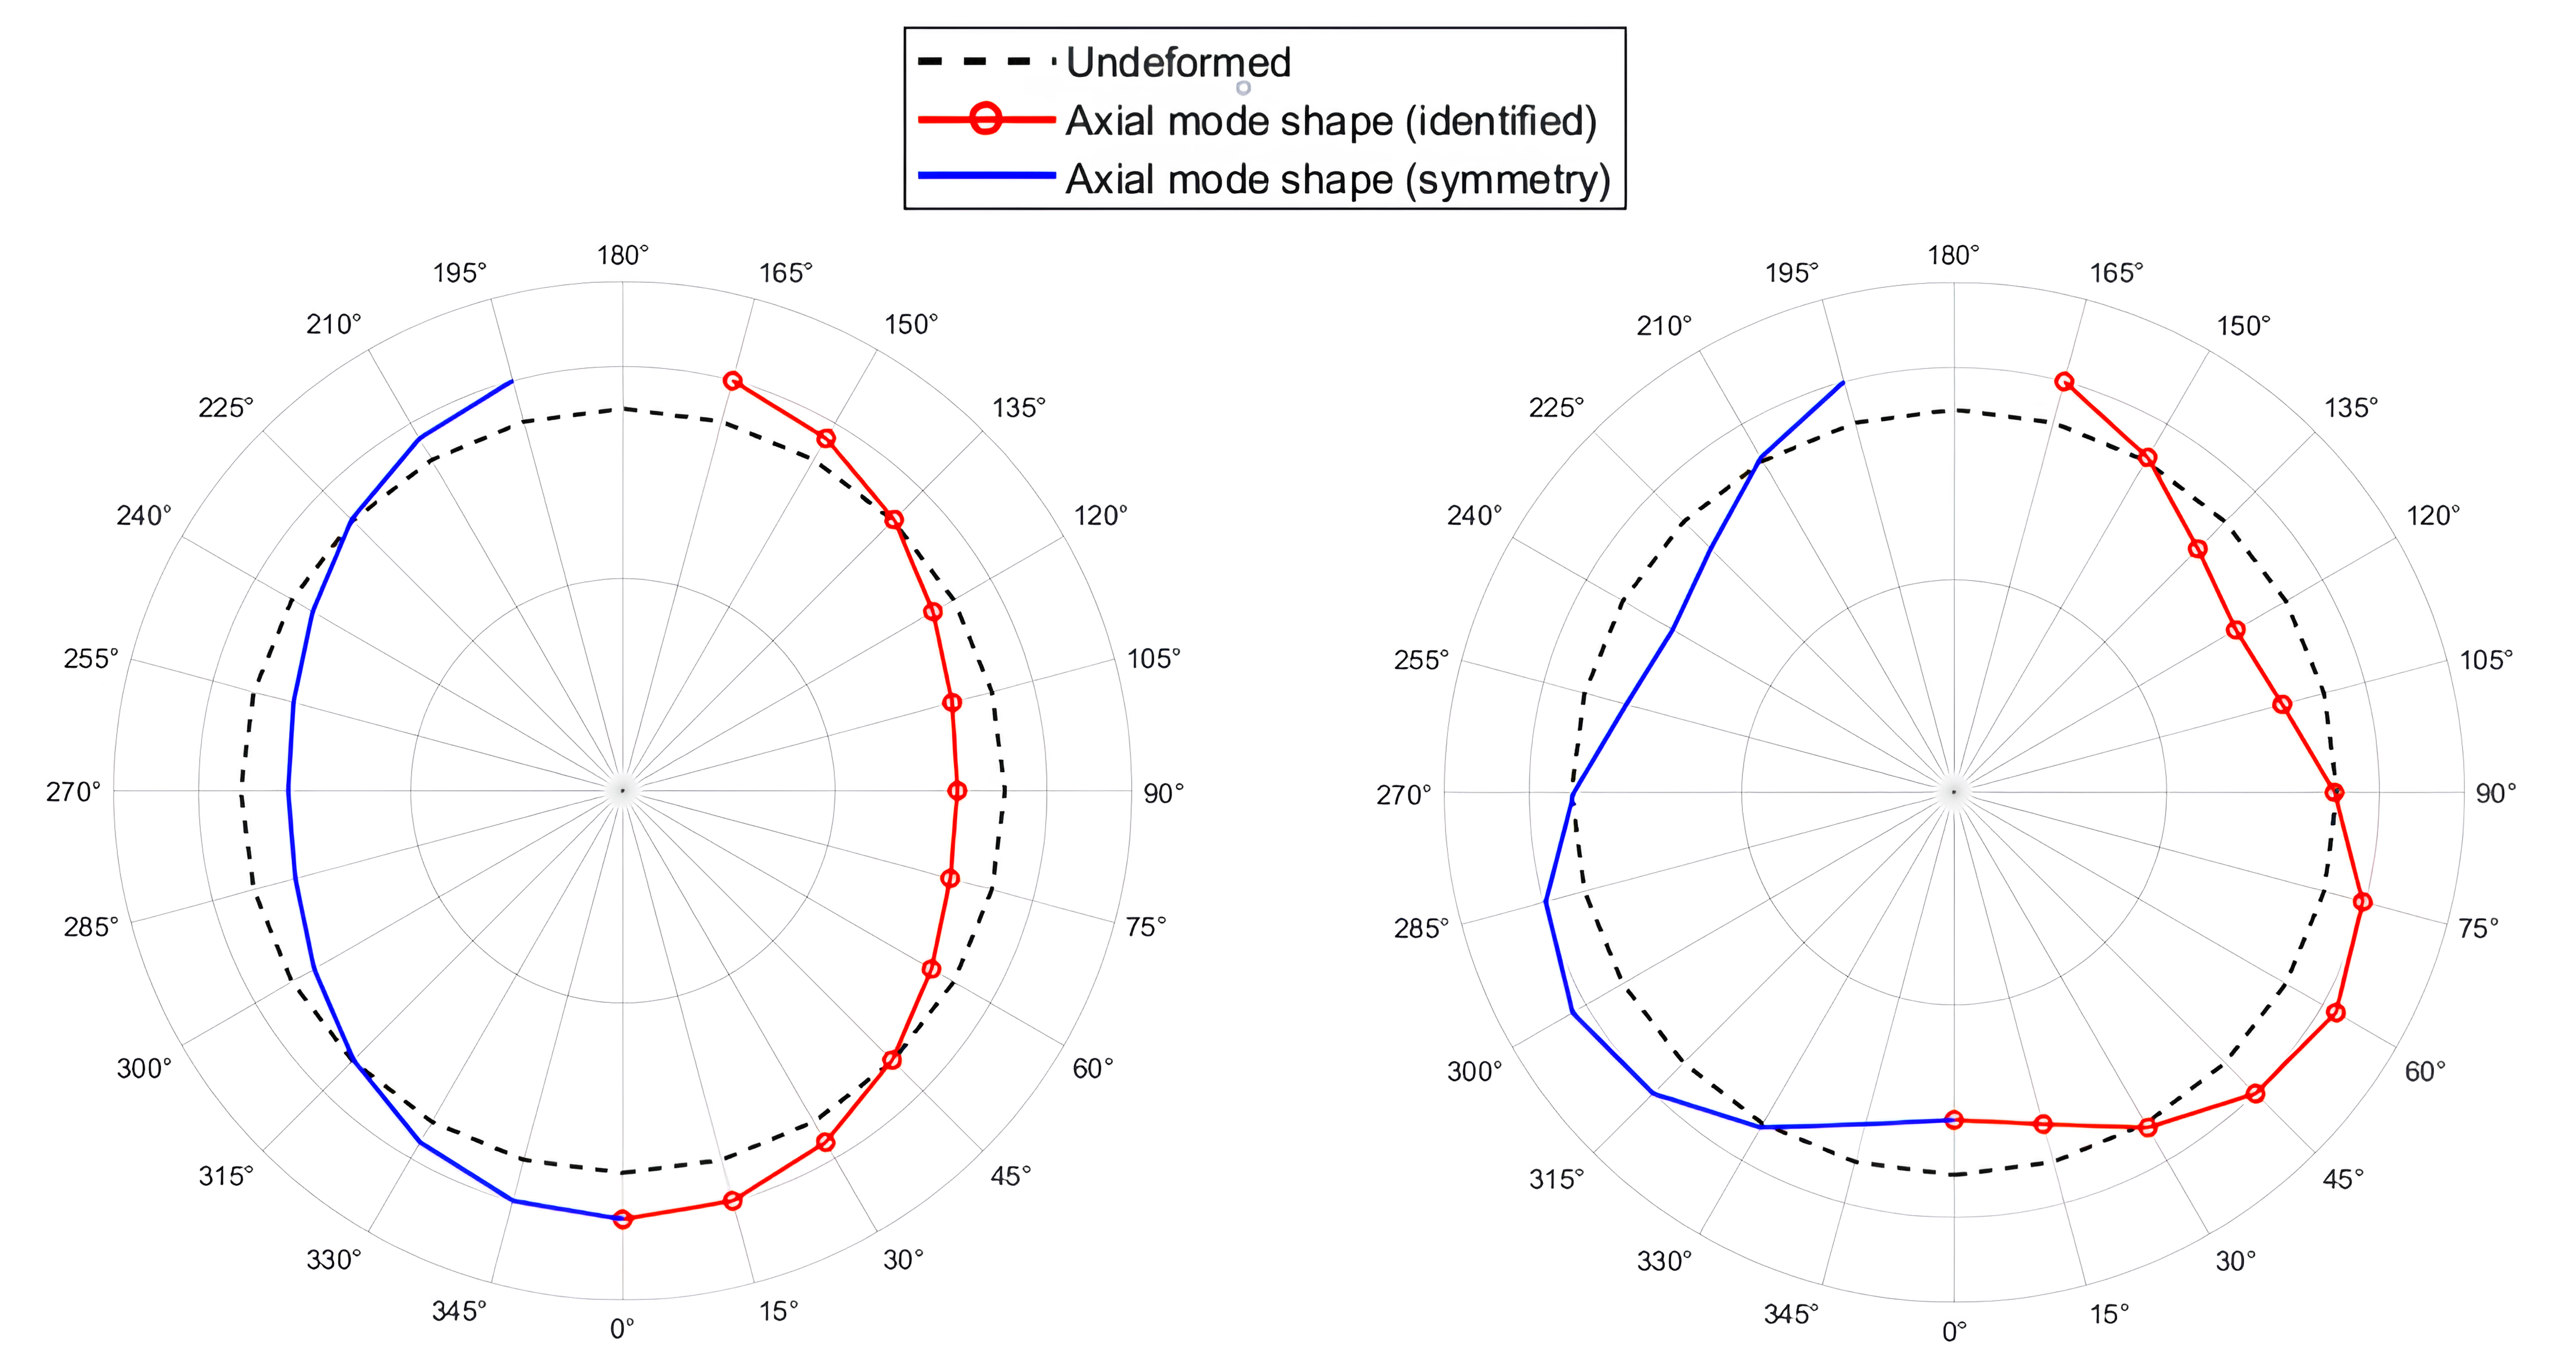
\includegraphics[scale=0.061]{Images/1 e 2 mode shapes.png}
    \caption{First and second axial mode shapes}
\end{figure}
\noindent Finally, the 12 points have been interpolated by means of a spline function, so that the curve is continuous to at least the second-order derivative at each point of the interval considered.\\
The interpolated mode shapes are reported below:
\begin{figure} [H]
    \centering
    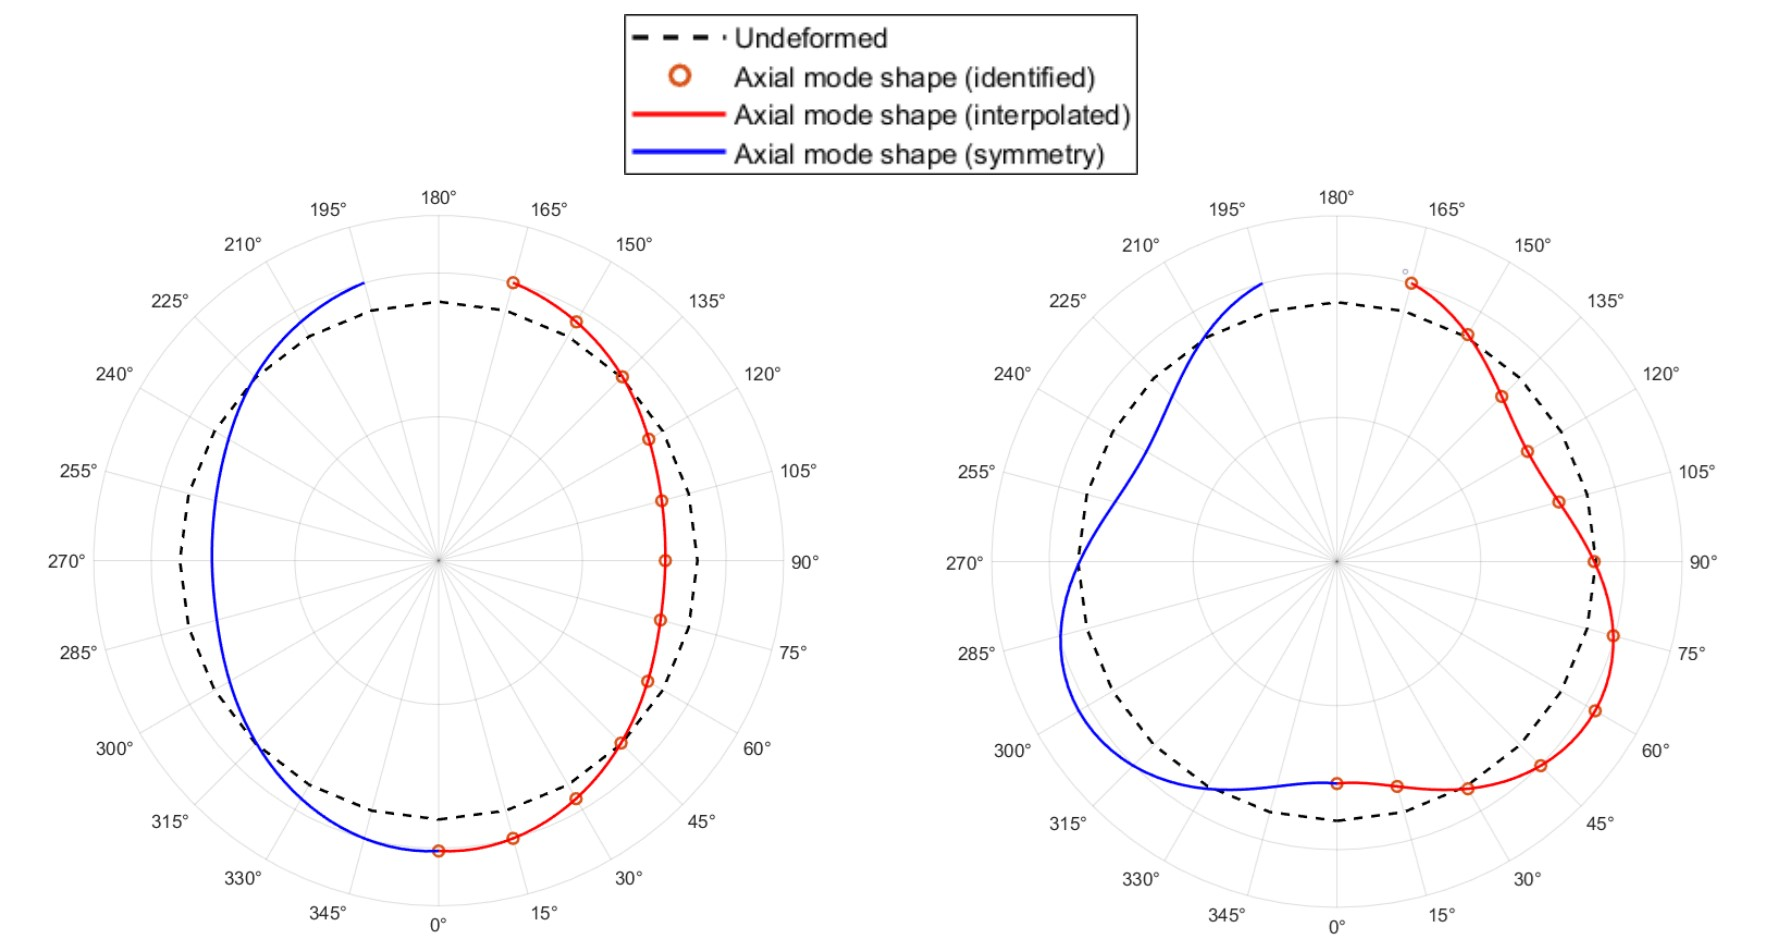
\includegraphics[scale=0.33]{Images/Interpolation.jpg}
    \caption{Interpolated first and second axial mode shapes}
\end{figure}

\end{document}
